\documentclass{oci}
\usepackage[utf8]{inputenc}
\usepackage{lipsum}
\usepackage{tikz}

\title{Cuatro en línea}

\begin{document}
\begin{problemDescription}
  El profesor de historia lleva una semana con
  licencia y la clase ha sido cancelada nuevamente.
  %
  Aburrida y sin tener mucho que hacer, Romina le
  propone a sus compañeras y compañeros hacer un torneo
  de cuatro en línea.

  El cuatro en línea es un juego de estrategia
  muy sencillo que se juega entre dos personas.
  %
  Para jugarlo solo se requiere un lápiz y una hoja de
  cuaderno cuadriculada.
  %
  El juego comienza definiendo una grilla de
  $N\times N$ sobre la hoja.
  %
  Posteriormente, los jugadores toman turnos
  marcado celdas en la grilla.
  %
  El primer jugador marca las celdas usando una
  \texttt{O} (la letra ``o'' mayúscula)
  y el segundo jugador marca sus celdas usando una
  \texttt{X} (la letra ``x'' mayúscula).
  %
  El objetivo de cada jugador es combinar \emph{cuatro celdas
  en línea}, es decir, cuatro celdas consecutivas de forma
  vertical, horizontal o diagonal.
  %
  En cada turno, un jugador puede marcar cualquier celda vacía
  dentro de la grilla.
  %
  El juego finaliza inmediatamente cuando alguno de los jugadores
  logra formar cuatro en línea.
  %
  Alternativamente, un juego puede terminar en empate si la grilla
  se llena completamente sin ninguno de los jugadores logrando
  cuatro en línea.
  %
  La siguiente figura muestra una posible secuencia de jugadas
  en una grilla de $4\times 4$ que resultan en el primer jugador
  victorioso al combinar cuatro \texttt{O}'s de forma diagonal.
  \begin{center}
  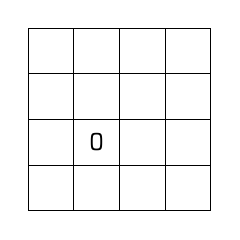
\begin{tikzpicture}[scale=0.58]
    \draw (0, 0) grid (4, 4);
    \node at (1.5, 1.5) {\texttt{O}};
  \end{tikzpicture}
  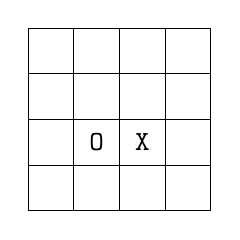
\begin{tikzpicture}[scale=0.58]
    \draw (0, 0) grid (4, 4);
    \node at (1.5, 1.5) {\texttt{O}};
    \node at (2.5, 1.5) {\texttt{X}};
  \end{tikzpicture}
  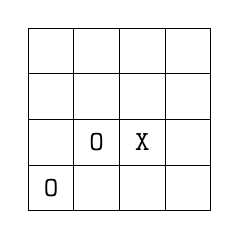
\begin{tikzpicture}[scale=0.58]
    \draw (0, 0) grid (4, 4);
    \node at (1.5, 1.5) {\texttt{O}};
    \node at (2.5, 1.5) {\texttt{X}};
    \node at (0.5, 0.5) {\texttt{O}};
  \end{tikzpicture}
  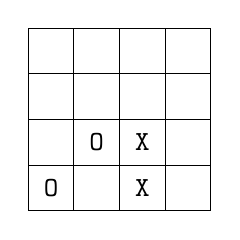
\begin{tikzpicture}[scale=0.58]
    \draw (0, 0) grid (4, 4);
    \node at (1.5, 1.5) {\texttt{O}};
    \node at (2.5, 1.5) {\texttt{X}};
    \node at (0.5, 0.5) {\texttt{O}};
    \node at (2.5, 0.5) {\texttt{X}};
  \end{tikzpicture}
  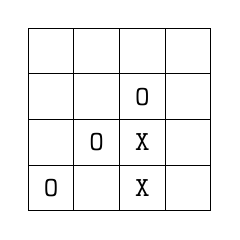
\begin{tikzpicture}[scale=0.58]
    \draw (0, 0) grid (4, 4);
    \node at (1.5, 1.5) {\texttt{O}};
    \node at (2.5, 1.5) {\texttt{X}};
    \node at (0.5, 0.5) {\texttt{O}};
    \node at (2.5, 0.5) {\texttt{X}};
    \node at (2.5, 2.5) {\texttt{O}};
  \end{tikzpicture}
  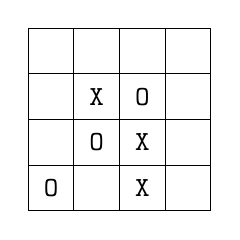
\begin{tikzpicture}[scale=0.58]
    \draw (0, 0) grid (4, 4);
    \node at (1.5, 1.5) {\texttt{O}};
    \node at (2.5, 1.5) {\texttt{X}};
    \node at (0.5, 0.5) {\texttt{O}};
    \node at (2.5, 0.5) {\texttt{X}};
    \node at (2.5, 2.5) {\texttt{O}};
    \node at (1.5, 2.5) {\texttt{X}};
  \end{tikzpicture}
  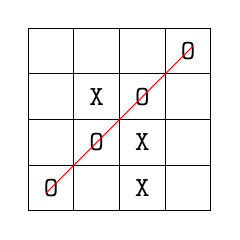
\begin{tikzpicture}[scale=0.58]
    \draw (0, 0) grid (4, 4);
    \node at (1.5, 1.5) {\texttt{O}};
    \node at (2.5, 1.5) {\texttt{X}};
    \node at (0.5, 0.5) {\texttt{O}};
    \node at (2.5, 0.5) {\texttt{X}};
    \node at (2.5, 2.5) {\texttt{O}};
    \node at (1.5, 2.5) {\texttt{X}};
    \node at (3.5, 3.5) {\texttt{O}};
    \draw[red] (0.4, 0.4) -- (3.6, 3.6);
  \end{tikzpicture}
  \end{center}

  Luego de terminar el torneo, Romina mira
  las grillas donde se jugó cada partida
  y sospecha que mucha gente no jugó en serio y
  simplemente marcó casillas sin seguir las reglas.
  %
  ?`Podrías ayudar a Romina a determinar si sus sospechas
  son ciertas?
  %
  Específicamente, dada una grilla donde algunas
  celdas han sido marcadas con una \texttt{O} o una \texttt{X}
  tu tarea es determinar si es posible que un juego de cuatro en
  línea termine con esta grilla.
\end{problemDescription}

\begin{inputDescription}
  La primera línea de la entrada contiene un entero $N$ ($4\leq N \leq 20$)
  correspondiente
  al tamaño de la grilla.
  %
  Posteriormente siguen $N$ líneas cada una conteniendo $N$ caracteres.
  %
  El carácter $j$-ésimo en la línea $i$-ésima corresponde al contenido
  de la celda en la fila $i$ y columna $j$.
  %
  El carácter será un punto si la casilla está vacía, o
  una \texttt{O} o una \texttt{X} si la casilla fue marcada.
\end{inputDescription}

\begin{outputDescription}
  La salida deber contener \texttt{posible} en caso de ser posible
  que siguiendo las reglas descritas en el enunciado la grilla en la
  entrada sea el resultado de un juego de cuatro en línea.
  %
  En caso de no ser posible la salida debe contener \texttt{imposible}.
\end{outputDescription}

\begin{scoreDescription}
  Este problema no contiene subtareas.
  Se otorgará puntaje de acuerdo a la cantidad de casos de prueba correctos siendo
  100 el puntaje máximo.
  %
  Para obtener puntaje mayor que cero debes tener al menos un 50\% de los casos
  correctos.
  %
  Específicamente, si $T$ es la cantidad total de casos y $C$ la cantidad de casos correctos,
  el puntaje será 0 si $C < \frac{T}{2}$.
  Si $C \geq \frac{T}{2}$, el puntaje será $\frac{2\cdot C - T}{T}\cdot 100$.
\end{scoreDescription}

\begin{sampleDescription}
\sampleIO{sample-1}
\sampleIO{sample-2}
\end{sampleDescription}

\end{document}
